% pdflatex -shell-escape software-analysis-main.tex
\documentclass[12pt,openany]{book}

\usepackage{kotex}
\usepackage{commath}
\usepackage{slantsc}
\usepackage{hyperref}
\usepackage{stmaryrd} %llbracket
\usepackage{adjustbox}
\usepackage{enumerate}

\usepackage{cite}
\usepackage[numbers]{natbib}
\usepackage{amsthm}

% Define custom theorem styles
\newtheoremstyle{dotless} % Name of the style
{3pt} % Space above
{3pt} % Space below
{\itshape} % Body font
{} % Indent amount
{\bfseries} % Theorem head font
{} % Punctuation after theorem head
{2.5mm} % Space after theorem head
{} % Theorem head spec

\newtheoremstyle{definitionstyle} % Name of the style
{3pt} % Space above
{3pt} % Space below
{} % Body font
{} % Indent amount
{\bfseries} % Theorem head font
{.} % Punctuation after theorem head
{2.5mm} % Space after theorem head
{} % Theorem head spec

% Applying custom styles
\theoremstyle{dotless}
\newtheorem{theorem}{Theorem}[section] % Theorem environment with section-wise numbering
\newtheorem{lemma}[theorem]{Lemma} % Lemma shares the counter with theorem
\newtheorem{corollary}[theorem]{Corollary} % Corollary shares the counter with theorem

\theoremstyle{definitionstyle}
\newtheorem{definition}[theorem]{Definition} % Definition shares the counter with theorem
\newtheorem{example}[theorem]{Example} % Example shares the counter with theorem
\newtheorem{remark}[theorem]{Remark} % Remark shares the counter with theorem
\newtheorem*{note}{Note}

% Colors
\usepackage[dvipsnames,table]{xcolor}
\definecolor{titleblue}{RGB}{0,53,128}
\definecolor{chaptergray}{RGB}{140,140,140}
\definecolor{sectiongray}{RGB}{180,180,180}

\definecolor{thmcolor}{RGB}{231, 76, 60}
\definecolor{defcolor}{RGB}{52, 152, 219}
\definecolor{lemcolor}{RGB}{155, 89, 182}
\definecolor{corcolor}{RGB}{46, 204, 113}
\definecolor{procolor}{RGB}{241, 196, 15}
\definecolor{execolor}{RGB}{90, 128, 127}

% Fonts
\usepackage[T1]{fontenc}
\usepackage[utf8]{inputenc}
\usepackage{newpxtext,newpxmath}
\usepackage{sectsty}
\allsectionsfont{\sffamily\color{titleblue}\mdseries}

% Page layout
\usepackage{geometry}
\geometry{a4paper,left=.8in,right=.6in,top=.75in,bottom=1in,heightrounded}
\usepackage{fancyhdr}
\fancyhf{}
\fancyhead[LE,RO]{\thepage}
\fancyhead[LO]{\nouppercase{\rightmark}}
\fancyhead[RE]{\nouppercase{\leftmark}}
\renewcommand{\headrulewidth}{0.5pt}
\renewcommand{\footrulewidth}{0pt}

% Chapter formatting
\usepackage{titlesec}
\titleformat{\chapter}[display]
{\normalfont\sffamily\Huge\bfseries\color{titleblue}}{\chaptertitlename\ \thechapter}{20pt}{\Huge}
\titleformat{\section}
{\normalfont\sffamily\Large\bfseries\color{titleblue!100!gray}}{\thesection}{1em}{}
\titleformat{\subsection}
{\normalfont\sffamily\large\bfseries\color{titleblue!75!gray}}{\thesubsection}{1em}{}

% Table of contents formatting
\usepackage{tocloft}
\renewcommand{\cftchapfont}{\sffamily\color{titleblue}\bfseries}
\renewcommand{\cftsecfont}{\sffamily\color{titleblue!100!gray}}
\renewcommand{\cftsubsecfont}{\sffamily\color{titleblue!75!gray}}
\renewcommand{\cftchapleader}{\cftdotfill{\cftdotsep}}

\usepackage{tikz}
\usepackage{tikz-cd}
\usetikzlibrary{shapes.geometric, arrows.meta, positioning}
\usepackage[ruled,linesnumbered]{algorithm2e}
\usepackage{setspace}
\usepackage{algpseudocode}
\SetKwComment{Comment}{/* }{ */}
\SetKw{Break}{break}
\SetKw{Downto}{downto}
\SetKwProg{Fn}{Function}{:}{end}
\SetKwProg{Procedure}{procedure}{:}{end}
\SetKwProg{Construct}{Construct}{:}{end}
\SetKwFunction{KeyGen}{KeyGen}

%Listing
\usepackage{listings} %Code
\renewcommand{\lstlistingname}{Code}%
\definecolor{keyword}{RGB}{255, 0, 0}
\definecolor{identifier}{RGB}{0, 0, 255}
\definecolor{comment}{RGB}{0, 128, 0}
\definecolor{string}{RGB}{163, 21, 21}

\lstdefinestyle{c}{
	language=C,
	basicstyle=\ttfamily\small,
	keywordstyle=\color{keyword},
	identifierstyle=\color{identifier},
	commentstyle=\color{comment}\itshape,
	stringstyle=\color{string},
	showstringspaces=false,
	%	numberstyle=\tiny\color{gray},
	%	numbersep=5pt,
	frame=single,
	tabsize=4,
	captionpos=b,
	breaklines=true,
	breakatwhitespace=true,
	%	numbers=left
}
\newcommand{\N}{\mathbb{N}}
\newcommand{\Z}{\mathbb{Z}}
\newcommand{\Q}{\mathbb{Q}}
\newcommand{\R}{\mathbb{R}}
\newcommand{\C}{\mathbb{C}}
\newcommand{\F}{\mathbb{F}}

\newcommand{\cP}{\mathcal{P}}
\newcommand{\cR}{\mathcal{R}}

\newcommand{\oracle}{\textsc{Oracle}}
\newcommand{\sub}[1]{\textsf{sub}\left(#1\right)}

\newcommand{\includecode}[2][c]{\lstinputlisting[caption=#2, escapechar=, style=C]{#2}<!---->}
%\input{cryptanalysis-lstlisting}
%\usepackage[backend=biber,style=numeric,citestyle=numeric]{biblatex}
%\addbibresource{swv-references.bib}
\begin{document}
	
	\begin{titlepage}
    \centering
    
    \vspace*{1cm}
    
    \Huge\textsf{\textbf{Software Verification}}
    
    \vspace{0.5cm}
    \LARGE\textsf{- A Deep Dive into Testing and Validation -}
    
    \vspace{1.5cm}
    \textbf{Ji, Yong-Hyeon}

    \vfill
    A document presented for\\
    the Software Verification
    
    \vspace{0.8cm}
    {\large\textsf{Department of Information Security, Cryptology, and Mathematics}\par}
    {\large\textsf{College of Science and Technology}\par}
    {\large\textsf{Kookmin University}\par}
    \vspace{.25in}
    {\large \textsf{\today}\par}
    
%    \Large{Institution Name}\\
%    Date
\end{titlepage}


	\tableofcontents
	\newpage
	\section*{Symbols}
In this paper, symbols are defined as follows. \\ \ \\ 
$
\begin{array}{cl}
	I\models P & \text{$I$ satisfies $P$} \\
	I\not\models P & \text{$I$ does not satisfies $P$} \\
\end{array}
$
	\newpage
	\chapter{Introduction}
	% Chapter I. Introduction

\cite{youtube:COSE419-Lecture1-1}
\cite{youtube:COSE419-Lecture1-2}
\cite{naver:bycho211-1}
	
	\newpage
%	\chapter{Greybox Fuzzing and Concolic Testing}
%	% Propositional Logic I

\cite{youtube:COSE419-Lecture4-1}

\section{Syntax and Semantic}
\subsection{Syntax}
\begin{itemize}
	\item \textbf{Atom}: basic elements
	\begin{itemize}
		\item truth symbols $\bot$(``false'') and $\top$(``true'')
		\item propositional variables $P,Q,R,\dots$
	\end{itemize}
	\item \textbf{Literal}: an atom $\alpha$ or its negation $\lnot\alpha$.
	\item \textbf{Formula}: a literal or the application of a logical connective (boolean connectives) to formulas
	\[
	\begin{array}{ccll}
		F & \to & \bot \\
		& | & \top \\
		& | & P \\
		& | & \lnot F & \text{negation (``not'')} \\
		& | & F_1\land F_2 & \text{conjunction (``and'')} \\
		& | & F_1\lor F_2 & \text{disjunction (``or'')} \\
		& | & F_1\to F_2 & \text{implication (``implies'')} \\
		& | & F_1\leftrightarrow F_2 & \text{iff (``if and only if'')}
	\end{array}
	\]
	\item[]
	\item Formula $G$ is a \textbf{subformula} of formula $F$ if it occurs syntactically within $G$.
	\begin{align*}
		\sub{\bot} &= \set{\bot} \\
		\sub{\top} &= \set{\top} \\
		\sub{P} &= \set{P} \\
		\sub{\lnot F} &= \set{\lnot F}\cup\sub{F} \\
		\sub{F_1\land F_2} &= \set{F_1\land F_2}\cup\sub{F_1}\cup\sub{F_2}
		&\vdots
	\end{align*}
	\item Consider $F:(P\land Q)\to (P\lor\lnot Q)$. Then \[
	\sub{F}=\set{F,P\land Q,P\lor\lnot Q,P,Q,\lnot Q}.
	\]
	\item The strict subformulas of a formula are all its subformulas except itself.
	\item[]
	\item To minimally use parentheses, we define the relative precedence of the logical connectives from highest to lowest as follows: \[
	\lnot\quad\land\quad\lor\quad\rightarrow\quad\leftrightarrow
	\]
	\item (Currying) Additionally, $\rightarrow$ and $\leftrightarrow$ associate to the right, e.g., \[
	P\to Q\to R\iff P\to(Q\to R).
	\]
	\item Example:
	\begin{itemize}
		\item $(P\land Q)\to (P\lor\lnot Q)\iff P\land Q\to P\lor \lnot Q$
		\item $(P_1\land((\lnot P_2)\land\top))\lor((\lnot P_1)\land P_2)\iff P_1\land P_2\top\lor\lnot P_1\land P_2$
	\end{itemize}
\end{itemize}

\subsection{Semantics}
\begin{itemize}
	\item The semantics of a logic provides its meaning. The meaning of a PL formula is either true or false.
	\item The semantics of a formula is defined with an \textbf{interpretation} (or assignment) that assigns truth values to propositional variables.
	\item For example, $F:P\land Q\to P\lor\land Q$ evaluates to true under the interpretation $I:\set{P\mapsto \text{true},Q\mapsto\text{false}}:$
	\begin{table}[h!]\centering\setstretch{1.25}
		\begin{tabular}{c|c||c|c|c|c}
			\hline
			$P$ & $Q$ & $\lnot Q$ & $P\land Q$ & $P\lor \lnot Q$ & $F$ \\ \hline
			1 & 0 & 1 & 0 & 1 & 1 \\ \hline
		\end{tabular}
	\end{table}
	\item The tabular notation is unsuitable for predicate logic. Instead, we define the semantics inductively.
\end{itemize}

\subsection{Inductive Definition of Semantics}
In an inductive definition, the meaning of basic elements is defined first.
The meaning of complex elements is defined in terms of subcomponents.
\begin{itemize}
	\item We write $I\models F$ if $F$ evaluates to \textbf{true} under $I$.
	\item We write $I\not\models F$ if $F$ evaluates to \textbf{false} under $I$.
\end{itemize}
Note that \[
\begin{array}{ll}
I\models \top,\quad I\not\models\bot, & \\
I\models P &\text{iff}\ I[P]=\text{true} \\
I\models \lnot F &\text{iff}\ I[P]=\text{false} \\
I\models\lnot F &\text{iff}\ I\not\models F \\
I\models F_1\land F_2 &\text{iff}\ I\models F_1\ \text{and}\ I\models F_2 \\
I\models F_1\lor F_2 &\text{iff}\ I\models F_1\ \text{or}\ I\models F_2 \\
I\models F_1\to F_2 &\text{iff}\ I\not\models F_1\ \text{or}\ I\models F_2 \\
I\models F_1\leftrightarrow F_2 &\text{iff}\ (I\models F_1\ \text{and}\ I\models F_2)\ \text{or}\ (I\not\models F_1\ \text{and}\ I\not\models F_2)
\end{array}
\]
\vspace{12pt}
\begin{example}
	Consider the formula \[
	F:P\land Q\to P\lor\lnot Q
	\] and the interpretation \[
	I:\set{P\mapsto\text{true},Q\mapsto\text{false}}.
	\] The truth value of $F$ is computed as follows: \[
	\begin{array}{ll}
		1.\quad I\models P &\text{since $I[P]=\text{true}$} \\
		2.\quad I\not\models Q &\text{since $I[P]=\text{true}$} \\
		3.\quad I\models \lnot Q &\text{by 2 and semantics of $\lnot$} \\
		4.\quad I\not\models P\land Q &\text{by 2 and semantics of $\land$} \\
		5.\quad I\models P\lor \lnot Q &\text{by 1 and semantics of $\lor$} \\
		6.\quad I\models F &\text{by 4 and semantics of $\to$} \\
	\end{array}
	\]
\end{example}

\section{Satisfiability and Validity}
\begin{itemize}
	\item A formula $F$ is \textbf{satisfiable} iff there exists an interpretation $I$ such that $I\models F$.
	\item A formula $F$ is \textbf{valid} iff for all interpretations $I$, $I\models F$.
	\item Satisfiability and validity are dual: \[
	\text{$F$ is valid}\iff\text{$\lnot F$ is unsatisfiable}
	\]
	\begin{proof}
		content...
	\end{proof}
	\item We can check satisfiability by deciding validity, and vice versa.
\end{itemize}

\begin{figure}[h!]\centering
\begin{tikzcd}
	& \text{VALID} \arrow[dr, "\neg"] & \\
	\text{SAT} \arrow[ur, "\neg"] \arrow[rr, "\neg"] & & \text{UNSAT} \\
	& \text{INVALID} \arrow[ul, "\neg"] \arrow[ur, "\neg"] &
\end{tikzcd}
\caption{Relation of SAT, UNSAT, VALID and INVALID}
\end{figure}

\begin{figure}[h!]\centering
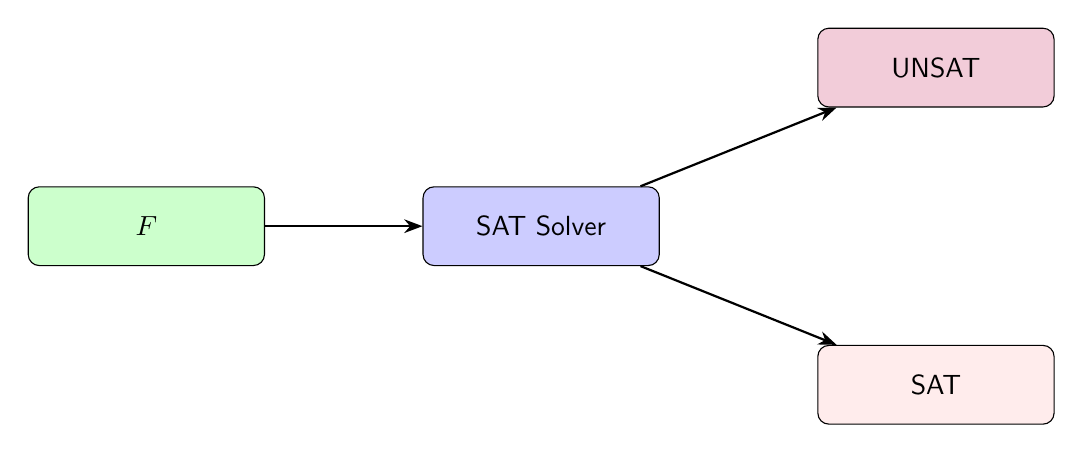
\begin{tikzpicture}[
	node distance=1cm and 2cm,
	process/.style={rectangle, rounded corners, draw, minimum width=3cm, minimum height=1cm, text centered, font=\sffamily},
	arrow/.style={-Stealth, thick},
	pastelgreen/.style={fill=green!20},
	pastelblue/.style={fill=blue!20},
	pastelpink/.style={fill=pink!30},
	pastelpurple/.style={fill=purple!20}
	]
	
	% Nodes
	\node (F) [process, pastelgreen] {$F$};
	\node (SATsolver) [process, pastelblue, right=of F] {SAT Solver};
	\node (SAT) [process, pastelpink, below right=of SATsolver] {SAT};
	\node (UNSAT) [process, pastelpurple, above right=of SATsolver] {UNSAT};
	
	% Arrows
	\draw[arrow] (F) -- (SATsolver);
	\draw[arrow] (SATsolver) -- node[below left] {} (SAT);
	\draw[arrow] (SATsolver) -- node[above left] {} (UNSAT);
	
\end{tikzpicture}
\end{figure}

\newpage
\subsection{Deciding Validity and Satisfiability}
Two approaches to show $F$ is valid:
\begin{itemize}
	\item \textbf{Truth Table Method} performs exhaustive search: e.g., \[
	F:P\land Q\to P\lor\lnot Q.
	\]
	\begin{table}[h!]\centering
		\begin{tabular}{c|c|c|c|c||c}
			\hline
			$P$ & $Q$ & $P\land Q$ & $\lnot Q$ & $P\lor\lnot Q$ & $F$ \\ \hline
			0 & 0 & 0 & 1 & 1 & 1 \\
			0 & 1 & 0 & 0 & 0 & 1 \\
			1 & 0 & 0 & 1 & 1 & 1 \\
			1 & 1 & 1 & 0 & 1 & 1 \\ \hline
		\end{tabular}
	\end{table} \\
	Non-applicable to logic with infinite domain (e.g., first-order logic).
	\item \textbf{Semantic Argument Method} uses deduction:
	\begin{itemize}
		\item Assume $F$ is valid: $I\not\models F$ for some $I$ (falsifying interpretation).
		\item Apply deduction rules (proof rules) to derive a contradiction.
		\item If every branch of the proof derives a contradiction, then $F$ is valid.
		\item If some branch of the proof never derives a contradiction, then $F$ is invalid.
	\end{itemize}
\end{itemize}

\subsection{Deduction Rules for Propositional Logic}
\begin{center}
\begin{minipage}{.48\textwidth}
	\item \textbf{Negation Elimination}\[
	\frac{I\models\lnot F}{I\not\models F}
	\] This rule shows how to derive $F$ from $\lnot F$. It eliminates the negation by asserting that if $\lnot F$ holds, then $F$ cannot hold.
	\vspace{12pt}
	\item \textbf{Conjunction Elimination}\footnote{And-Elimination}\[
	\frac{I\models F\land G}{I\models F, I\models G}
	\] This rule breaks down a conjunction into its individual components, showing that if 
	$F\land G$ is true, then both $F$ and $G$ are true.
	\vspace{12pt}
	\item \textbf{Disjunction Elimination}\footnote{Or-Elimination} \[
	\frac{I\models F\lor G}{I\models F\mid I\models G}
	\] This rule asserts that if $F\lor G$ is true in an interpretation, then either 
	$F$ is true, or $G$ is true, or both are true. This is also sometimes referred to as the rule of cases.
	\vspace{12pt}
	\item \textbf{Implication Elimination}\footnote{Material Implication}\[
	\frac{I\models F\to G}{I\not\models F\mid I\models G}
	\] This rule states that if $F\to G$ is true in an interpretation, then either 
	$F$ is false or $G$ is true. This corresponds to the definition of material implication in classical logic.
	
	\vspace{12pt}
	\item \textbf{Biconditional Elimination}\footnote{If and Only If Elimination}\[
	\frac{I\models F\leftrightarrow G}{I\models F\land G\mid I\models\lnot F\land\lnot G}
	\] This rule states that if $F\leftrightarrow G$ is true in an interpretation, then either both 
	$F$ and $G$ are true, or both $F$ and $G$ are false. This corresponds to the definition of a biconditional statement in classical logic.
\end{minipage}\quad
\begin{minipage}{.48\textwidth}
\item \textbf{Negation Introduction} \[
\frac{I\not\models \lnot F}{I\models F}
\] This rule introduces $F$ from the fact that $\lnot F$ does not hold. It asserts that if the negation of $F$ does not hold, then $F$ must hold.
\vspace{12pt}
\item \textbf{De Morgan's Law for Conjunction}\footnote{Contrapositive of Conjunction Introduction}\[
\frac{I\not\models F\land G}{I\not\models F \mid I\not\models G}
\] This rule states that if 
$F\land G$ is not true, then at least one of $F$ or $G$ is not true. This is an application of De Morgan's laws.
\vspace{12pt}
\item \textbf{De Morgan's Law for Disjunction}\footnote{Contrapositive of Disjunction Introduction}\[
\frac{I\not\models F\lor G}{I\not\models F, I\not\models G}
\] This rule states that if $F\lor G$ is not true, then both $F$ is not true and $G$ is not true.  This is directly derived from De Morgan's laws in classical logic.
\vspace{12pt}
\item \textbf{Denial of Implication}\footnote{Contrapositive of Implication} \[
\frac{I\not\models F\to G}{I\models F, I\not\models G}
\] This rule states that if $F\to G$ is not true in an interpretation, then 
$F$ must be true and $G$ must be false. This is the contrapositive form of material implication.
\vspace{12pt}
\item \textbf{Negation of Biconditional}\footnote{Exclusive Or Elimination} \[
\frac{I\not\models F\leftrightarrow G}{I\models F\land \lnot G\mid I\models\lnot F\land G}
\] This rule states that if $F\leftrightarrow G$ is not true in an interpretation, then $F$ and 
$G$ have opposite truth values, i.e., either $F$ is true and $G$ is false, or $F$ is false and $G$ is true.
This aligns with the concept of exclusive or (XOR).
\end{minipage}
\end{center}
\begin{center}
\textbf{Contradiction Introduction} (Proof by Contradiction) \[
\frac{I\models F\quad I\not\models F}{I\models\bot}
\]
\end{center}
\begin{example}
	To prove that the formula \[
	F:P\land Q\to P\lor\lnot Q
	\] is valid, assume that it is invalid and derive a contradiction:
	\[
	\begin{array}{ll}
		1.\quad I\not\models P\land \to P\lor\lnot Q & \text{assumption} \\
		2.\quad I\models P\land Q & \text{by 1 and semantics of $\to$} \\
		3.\quad I\not\models P\lor \lnot Q & \text{by 1 and semantics of $\to$} \\
		4.\quad I\models P & \text{by 2 and semantics of $\land$} \\
		5.\quad I\lnot\models P & \text{by 3 and semantics of $\lor$} \\
		6.\quad I\models\bot & \text{4 and 5 are contradictory}
	\end{array}
	\]
\end{example}

\begin{example}
	To prove that the formula \[
	F:(P\to Q)\land(Q\to R)\to(P\to R)
	\] is valid, assume that it is invalid and derive a contradiction:
\end{example}

\subsection{Proof Tree}

\subsection{Derived Rules}


%\subsection*{1. Modus Ponens (MP)}
%\[
%\frac{A, \quad A \rightarrow B}{B}
%\]
%
%\subsection*{2. Modus Tollens (MT)}
%\[
%\frac{A \rightarrow B, \quad \neg B}{\neg A}
%\]
%
%\subsection*{3. Disjunction Introduction (DI)}
%\[
%\frac{A}{A \vee B}
%\]
%\[
%\frac{B}{A \vee B}
%\]
%
%\subsection*{4. Disjunction Elimination (DE)}
%\[
%\frac{A \vee B, \quad \neg A}{B}
%\]
%\[
%\frac{A \vee B, \quad \neg B}{A}
%\]
%
%\subsection*{5. Conjunction Introduction (CI)}
%\[
%\frac{A, \quad B}{A \wedge B}
%\]
%
%\subsection*{6. Conjunction Elimination (CE)}
%\[
%\frac{A \wedge B}{A}
%\]
%\[
%\frac{A \wedge B}{B}
%\]
%
%\subsection*{7. Biconditional Introduction (BI)}
%\[
%\frac{A \rightarrow B, \quad B \rightarrow A}{A \leftrightarrow B}
%\]
%
%\subsection*{8. Biconditional Elimination (BE)}
%\[
%\frac{A \leftrightarrow B}{A \rightarrow B}
%\]
%\[
%\frac{A \leftrightarrow B}{B \rightarrow A}
%\]
%
%\subsection*{9. Negation Introduction (NI)}
%\[
%\frac{A \rightarrow \bot}{\neg A}
%\]
%
%\subsection*{10. Negation Elimination (NE)}
%\[
%\frac{\neg A \rightarrow \bot}{A}
%\]
%
%\subsection*{11. Double Negation Elimination (DNE)}
%\[
%\frac{\neg \neg A}{A}
%\]
%
%\subsection*{12. Contradiction Elimination (CE)}
%\[
%\frac{\bot}{A}
%\]
%
%\subsection*{13. Contradiction Introduction (CI)}
%\[
%\frac{A \wedge \neg A}{\bot}
%\]
	
	\newpage
	\chapter{Propositional Logic I}
	% Propositional Logic I

\cite{youtube:COSE419-Lecture4-1}

\section{Syntax and Semantic}
\subsection{Syntax}
\begin{itemize}
	\item \textbf{Atom}: basic elements
	\begin{itemize}
		\item truth symbols $\bot$(``false'') and $\top$(``true'')
		\item propositional variables $P,Q,R,\dots$
	\end{itemize}
	\item \textbf{Literal}: an atom $\alpha$ or its negation $\lnot\alpha$.
	\item \textbf{Formula}: a literal or the application of a logical connective (boolean connectives) to formulas
	\[
	\begin{array}{ccll}
		F & \to & \bot \\
		& | & \top \\
		& | & P \\
		& | & \lnot F & \text{negation (``not'')} \\
		& | & F_1\land F_2 & \text{conjunction (``and'')} \\
		& | & F_1\lor F_2 & \text{disjunction (``or'')} \\
		& | & F_1\to F_2 & \text{implication (``implies'')} \\
		& | & F_1\leftrightarrow F_2 & \text{iff (``if and only if'')}
	\end{array}
	\]
	\item[]
	\item Formula $G$ is a \textbf{subformula} of formula $F$ if it occurs syntactically within $G$.
	\begin{align*}
		\sub{\bot} &= \set{\bot} \\
		\sub{\top} &= \set{\top} \\
		\sub{P} &= \set{P} \\
		\sub{\lnot F} &= \set{\lnot F}\cup\sub{F} \\
		\sub{F_1\land F_2} &= \set{F_1\land F_2}\cup\sub{F_1}\cup\sub{F_2}
		&\vdots
	\end{align*}
	\item Consider $F:(P\land Q)\to (P\lor\lnot Q)$. Then \[
	\sub{F}=\set{F,P\land Q,P\lor\lnot Q,P,Q,\lnot Q}.
	\]
	\item The strict subformulas of a formula are all its subformulas except itself.
	\item[]
	\item To minimally use parentheses, we define the relative precedence of the logical connectives from highest to lowest as follows: \[
	\lnot\quad\land\quad\lor\quad\rightarrow\quad\leftrightarrow
	\]
	\item (Currying) Additionally, $\rightarrow$ and $\leftrightarrow$ associate to the right, e.g., \[
	P\to Q\to R\iff P\to(Q\to R).
	\]
	\item Example:
	\begin{itemize}
		\item $(P\land Q)\to (P\lor\lnot Q)\iff P\land Q\to P\lor \lnot Q$
		\item $(P_1\land((\lnot P_2)\land\top))\lor((\lnot P_1)\land P_2)\iff P_1\land P_2\top\lor\lnot P_1\land P_2$
	\end{itemize}
\end{itemize}

\subsection{Semantics}
\begin{itemize}
	\item The semantics of a logic provides its meaning. The meaning of a PL formula is either true or false.
	\item The semantics of a formula is defined with an \textbf{interpretation} (or assignment) that assigns truth values to propositional variables.
	\item For example, $F:P\land Q\to P\lor\land Q$ evaluates to true under the interpretation $I:\set{P\mapsto \text{true},Q\mapsto\text{false}}:$
	\begin{table}[h!]\centering\setstretch{1.25}
		\begin{tabular}{c|c||c|c|c|c}
			\hline
			$P$ & $Q$ & $\lnot Q$ & $P\land Q$ & $P\lor \lnot Q$ & $F$ \\ \hline
			1 & 0 & 1 & 0 & 1 & 1 \\ \hline
		\end{tabular}
	\end{table}
	\item The tabular notation is unsuitable for predicate logic. Instead, we define the semantics inductively.
\end{itemize}

\subsection{Inductive Definition of Semantics}
In an inductive definition, the meaning of basic elements is defined first.
The meaning of complex elements is defined in terms of subcomponents.
\begin{itemize}
	\item We write $I\models F$ if $F$ evaluates to \textbf{true} under $I$.
	\item We write $I\not\models F$ if $F$ evaluates to \textbf{false} under $I$.
\end{itemize}
Note that \[
\begin{array}{ll}
I\models \top,\quad I\not\models\bot, & \\
I\models P &\text{iff}\ I[P]=\text{true} \\
I\models \lnot F &\text{iff}\ I[P]=\text{false} \\
I\models\lnot F &\text{iff}\ I\not\models F \\
I\models F_1\land F_2 &\text{iff}\ I\models F_1\ \text{and}\ I\models F_2 \\
I\models F_1\lor F_2 &\text{iff}\ I\models F_1\ \text{or}\ I\models F_2 \\
I\models F_1\to F_2 &\text{iff}\ I\not\models F_1\ \text{or}\ I\models F_2 \\
I\models F_1\leftrightarrow F_2 &\text{iff}\ (I\models F_1\ \text{and}\ I\models F_2)\ \text{or}\ (I\not\models F_1\ \text{and}\ I\not\models F_2)
\end{array}
\]
\vspace{12pt}
\begin{example}
	Consider the formula \[
	F:P\land Q\to P\lor\lnot Q
	\] and the interpretation \[
	I:\set{P\mapsto\text{true},Q\mapsto\text{false}}.
	\] The truth value of $F$ is computed as follows: \[
	\begin{array}{ll}
		1.\quad I\models P &\text{since $I[P]=\text{true}$} \\
		2.\quad I\not\models Q &\text{since $I[P]=\text{true}$} \\
		3.\quad I\models \lnot Q &\text{by 2 and semantics of $\lnot$} \\
		4.\quad I\not\models P\land Q &\text{by 2 and semantics of $\land$} \\
		5.\quad I\models P\lor \lnot Q &\text{by 1 and semantics of $\lor$} \\
		6.\quad I\models F &\text{by 4 and semantics of $\to$} \\
	\end{array}
	\]
\end{example}

\section{Satisfiability and Validity}
\begin{itemize}
	\item A formula $F$ is \textbf{satisfiable} iff there exists an interpretation $I$ such that $I\models F$.
	\item A formula $F$ is \textbf{valid} iff for all interpretations $I$, $I\models F$.
	\item Satisfiability and validity are dual: \[
	\text{$F$ is valid}\iff\text{$\lnot F$ is unsatisfiable}
	\]
	\begin{proof}
		content...
	\end{proof}
	\item We can check satisfiability by deciding validity, and vice versa.
\end{itemize}

\begin{figure}[h!]\centering
\begin{tikzcd}
	& \text{VALID} \arrow[dr, "\neg"] & \\
	\text{SAT} \arrow[ur, "\neg"] \arrow[rr, "\neg"] & & \text{UNSAT} \\
	& \text{INVALID} \arrow[ul, "\neg"] \arrow[ur, "\neg"] &
\end{tikzcd}
\caption{Relation of SAT, UNSAT, VALID and INVALID}
\end{figure}

\begin{figure}[h!]\centering
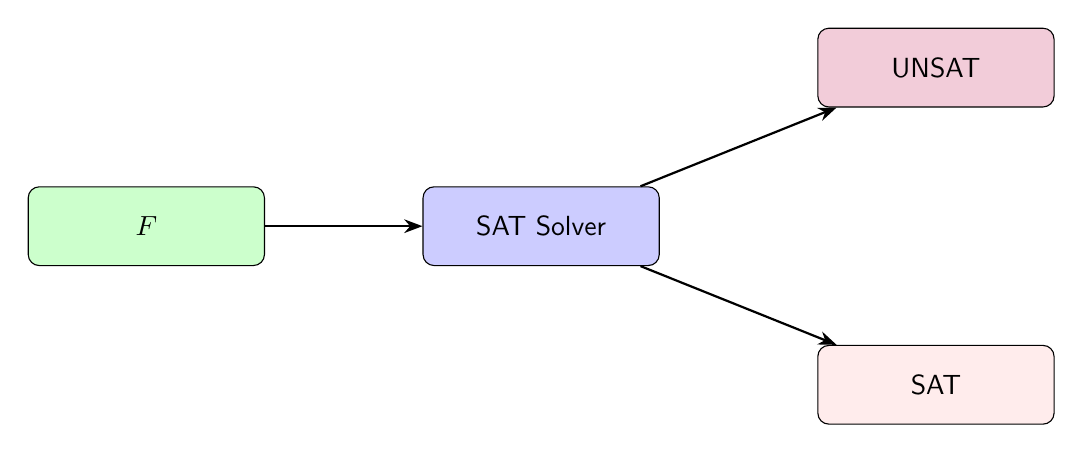
\begin{tikzpicture}[
	node distance=1cm and 2cm,
	process/.style={rectangle, rounded corners, draw, minimum width=3cm, minimum height=1cm, text centered, font=\sffamily},
	arrow/.style={-Stealth, thick},
	pastelgreen/.style={fill=green!20},
	pastelblue/.style={fill=blue!20},
	pastelpink/.style={fill=pink!30},
	pastelpurple/.style={fill=purple!20}
	]
	
	% Nodes
	\node (F) [process, pastelgreen] {$F$};
	\node (SATsolver) [process, pastelblue, right=of F] {SAT Solver};
	\node (SAT) [process, pastelpink, below right=of SATsolver] {SAT};
	\node (UNSAT) [process, pastelpurple, above right=of SATsolver] {UNSAT};
	
	% Arrows
	\draw[arrow] (F) -- (SATsolver);
	\draw[arrow] (SATsolver) -- node[below left] {} (SAT);
	\draw[arrow] (SATsolver) -- node[above left] {} (UNSAT);
	
\end{tikzpicture}
\end{figure}

\newpage
\subsection{Deciding Validity and Satisfiability}
Two approaches to show $F$ is valid:
\begin{itemize}
	\item \textbf{Truth Table Method} performs exhaustive search: e.g., \[
	F:P\land Q\to P\lor\lnot Q.
	\]
	\begin{table}[h!]\centering
		\begin{tabular}{c|c|c|c|c||c}
			\hline
			$P$ & $Q$ & $P\land Q$ & $\lnot Q$ & $P\lor\lnot Q$ & $F$ \\ \hline
			0 & 0 & 0 & 1 & 1 & 1 \\
			0 & 1 & 0 & 0 & 0 & 1 \\
			1 & 0 & 0 & 1 & 1 & 1 \\
			1 & 1 & 1 & 0 & 1 & 1 \\ \hline
		\end{tabular}
	\end{table} \\
	Non-applicable to logic with infinite domain (e.g., first-order logic).
	\item \textbf{Semantic Argument Method} uses deduction:
	\begin{itemize}
		\item Assume $F$ is valid: $I\not\models F$ for some $I$ (falsifying interpretation).
		\item Apply deduction rules (proof rules) to derive a contradiction.
		\item If every branch of the proof derives a contradiction, then $F$ is valid.
		\item If some branch of the proof never derives a contradiction, then $F$ is invalid.
	\end{itemize}
\end{itemize}

\subsection{Deduction Rules for Propositional Logic}
\begin{center}
\begin{minipage}{.48\textwidth}
	\item \textbf{Negation Elimination}\[
	\frac{I\models\lnot F}{I\not\models F}
	\] This rule shows how to derive $F$ from $\lnot F$. It eliminates the negation by asserting that if $\lnot F$ holds, then $F$ cannot hold.
	\vspace{12pt}
	\item \textbf{Conjunction Elimination}\footnote{And-Elimination}\[
	\frac{I\models F\land G}{I\models F, I\models G}
	\] This rule breaks down a conjunction into its individual components, showing that if 
	$F\land G$ is true, then both $F$ and $G$ are true.
	\vspace{12pt}
	\item \textbf{Disjunction Elimination}\footnote{Or-Elimination} \[
	\frac{I\models F\lor G}{I\models F\mid I\models G}
	\] This rule asserts that if $F\lor G$ is true in an interpretation, then either 
	$F$ is true, or $G$ is true, or both are true. This is also sometimes referred to as the rule of cases.
	\vspace{12pt}
	\item \textbf{Implication Elimination}\footnote{Material Implication}\[
	\frac{I\models F\to G}{I\not\models F\mid I\models G}
	\] This rule states that if $F\to G$ is true in an interpretation, then either 
	$F$ is false or $G$ is true. This corresponds to the definition of material implication in classical logic.
	
	\vspace{12pt}
	\item \textbf{Biconditional Elimination}\footnote{If and Only If Elimination}\[
	\frac{I\models F\leftrightarrow G}{I\models F\land G\mid I\models\lnot F\land\lnot G}
	\] This rule states that if $F\leftrightarrow G$ is true in an interpretation, then either both 
	$F$ and $G$ are true, or both $F$ and $G$ are false. This corresponds to the definition of a biconditional statement in classical logic.
\end{minipage}\quad
\begin{minipage}{.48\textwidth}
\item \textbf{Negation Introduction} \[
\frac{I\not\models \lnot F}{I\models F}
\] This rule introduces $F$ from the fact that $\lnot F$ does not hold. It asserts that if the negation of $F$ does not hold, then $F$ must hold.
\vspace{12pt}
\item \textbf{De Morgan's Law for Conjunction}\footnote{Contrapositive of Conjunction Introduction}\[
\frac{I\not\models F\land G}{I\not\models F \mid I\not\models G}
\] This rule states that if 
$F\land G$ is not true, then at least one of $F$ or $G$ is not true. This is an application of De Morgan's laws.
\vspace{12pt}
\item \textbf{De Morgan's Law for Disjunction}\footnote{Contrapositive of Disjunction Introduction}\[
\frac{I\not\models F\lor G}{I\not\models F, I\not\models G}
\] This rule states that if $F\lor G$ is not true, then both $F$ is not true and $G$ is not true.  This is directly derived from De Morgan's laws in classical logic.
\vspace{12pt}
\item \textbf{Denial of Implication}\footnote{Contrapositive of Implication} \[
\frac{I\not\models F\to G}{I\models F, I\not\models G}
\] This rule states that if $F\to G$ is not true in an interpretation, then 
$F$ must be true and $G$ must be false. This is the contrapositive form of material implication.
\vspace{12pt}
\item \textbf{Negation of Biconditional}\footnote{Exclusive Or Elimination} \[
\frac{I\not\models F\leftrightarrow G}{I\models F\land \lnot G\mid I\models\lnot F\land G}
\] This rule states that if $F\leftrightarrow G$ is not true in an interpretation, then $F$ and 
$G$ have opposite truth values, i.e., either $F$ is true and $G$ is false, or $F$ is false and $G$ is true.
This aligns with the concept of exclusive or (XOR).
\end{minipage}
\end{center}
\begin{center}
\textbf{Contradiction Introduction} (Proof by Contradiction) \[
\frac{I\models F\quad I\not\models F}{I\models\bot}
\]
\end{center}
\begin{example}
	To prove that the formula \[
	F:P\land Q\to P\lor\lnot Q
	\] is valid, assume that it is invalid and derive a contradiction:
	\[
	\begin{array}{ll}
		1.\quad I\not\models P\land \to P\lor\lnot Q & \text{assumption} \\
		2.\quad I\models P\land Q & \text{by 1 and semantics of $\to$} \\
		3.\quad I\not\models P\lor \lnot Q & \text{by 1 and semantics of $\to$} \\
		4.\quad I\models P & \text{by 2 and semantics of $\land$} \\
		5.\quad I\lnot\models P & \text{by 3 and semantics of $\lor$} \\
		6.\quad I\models\bot & \text{4 and 5 are contradictory}
	\end{array}
	\]
\end{example}

\begin{example}
	To prove that the formula \[
	F:(P\to Q)\land(Q\to R)\to(P\to R)
	\] is valid, assume that it is invalid and derive a contradiction:
\end{example}

\subsection{Proof Tree}

\subsection{Derived Rules}


%\subsection*{1. Modus Ponens (MP)}
%\[
%\frac{A, \quad A \rightarrow B}{B}
%\]
%
%\subsection*{2. Modus Tollens (MT)}
%\[
%\frac{A \rightarrow B, \quad \neg B}{\neg A}
%\]
%
%\subsection*{3. Disjunction Introduction (DI)}
%\[
%\frac{A}{A \vee B}
%\]
%\[
%\frac{B}{A \vee B}
%\]
%
%\subsection*{4. Disjunction Elimination (DE)}
%\[
%\frac{A \vee B, \quad \neg A}{B}
%\]
%\[
%\frac{A \vee B, \quad \neg B}{A}
%\]
%
%\subsection*{5. Conjunction Introduction (CI)}
%\[
%\frac{A, \quad B}{A \wedge B}
%\]
%
%\subsection*{6. Conjunction Elimination (CE)}
%\[
%\frac{A \wedge B}{A}
%\]
%\[
%\frac{A \wedge B}{B}
%\]
%
%\subsection*{7. Biconditional Introduction (BI)}
%\[
%\frac{A \rightarrow B, \quad B \rightarrow A}{A \leftrightarrow B}
%\]
%
%\subsection*{8. Biconditional Elimination (BE)}
%\[
%\frac{A \leftrightarrow B}{A \rightarrow B}
%\]
%\[
%\frac{A \leftrightarrow B}{B \rightarrow A}
%\]
%
%\subsection*{9. Negation Introduction (NI)}
%\[
%\frac{A \rightarrow \bot}{\neg A}
%\]
%
%\subsection*{10. Negation Elimination (NE)}
%\[
%\frac{\neg A \rightarrow \bot}{A}
%\]
%
%\subsection*{11. Double Negation Elimination (DNE)}
%\[
%\frac{\neg \neg A}{A}
%\]
%
%\subsection*{12. Contradiction Elimination (CE)}
%\[
%\frac{\bot}{A}
%\]
%
%\subsection*{13. Contradiction Introduction (CI)}
%\[
%\frac{A \wedge \neg A}{\bot}
%\]
	
	\newpage
	\chapter{Propositional Logic II}
	% Propositional Logic II

\cite{youtube:COSE419-Lecture4-1}
\cite{youtube:COSE419-Lecture4-2}
\cite{youtube:COSE419-Lecture4-3}

\section{Equivalence and Implication, and Equisatisfiability}

\section{Substitution}

\section{Normal Forms: NNF, DNF, CNF}

\subsection{Negation Normal Form (NNF)}
\subsection{Disjunctive Normal Form (DNF)}
\subsection{Conjunctive Normal Form (CNF)}

\section{Decision Procedures for Satisfiability}

%\section{Substitution}
%
%\section{Semantic Consequences of Substitution}
%
%\section{Composition of Substitutions}
%
%\section{Normal Form}

%
%\section{Decision Procedures}
%
%\section{Exhaustive Search}
%
%\section{DPLL}
%
%\section{Equisatisfiability}
%
%\section{Conversion to an Equisatisfiable Formula in CNF}
%
%\section{The Resolution Procedure}
%
%\section{Pure Literal Elimination (PLE)}
	
	\newpage
	\chapter{Problem Solving using SMT Solver}
	% Problem Solving using SMT Solver

\cite{youtube:COSE419-Lecture5-1}
\cite{youtube:COSE419-Lecture5-2}
\cite{youtube:COSE419-Lecture5-3}
	
	\newpage
	\chapter{First-Order Logic}
	% First-Order Logic

\section{Syntax and Semantics of FOL}

\section{Satisfiability and Validity}

\section{Substitution}

\section{Normal Forms}

\section{Soundness, Completeness, and Decidability}

\section{First-Order Theories}
	
	%
	%\chapter{Preliminaries}
	%\input{preliminaries.tex}
	
%	\chapter{Midterm Examination}
%	\input{cryptanalysis-contents/cryptanalysis-ch1-midterm}
	
%	\chapter{Practice Code}
%	\input{cryptanalysis-contents/cryptanalysis-src1-tmto}
	%\input{cryptanalysis-contents/cryptanalysis-ch2-tmto}
	% Add more topics as needed
	
%	\newpage
%	\printbibliography
%	\input{bibliography.tex}
	
%	\footnotesize
	\bibliographystyle{plain}
%	\bibliographystyle{plainnat}  % Use the plainnat style
	\bibliography{swv-references}
	
\end{document}
